\chapter{Merging algorithm}
\label{chap:mergingalgorithm}

% TODO add visualisation

This section presents an algorithm for estimating transformations between $n$ maps and merging them together. As discussed in the chapter~\ref{chap:analysis}, we work with maps represented as point clouds, possibly with \gls{RGB} information for each point.

There are two core problems for estimating the transformations. First we need to be able to estimate pair-wise transformation for $2$ maps using only geometrical and possibly colour information available within point clouds. We discuss our method in the section~\ref{sec:estimate-pair-wise}. Second, we want to get a transformation for each of the maps to the selected reference frame. This is discussed in the section~\ref{sec:estimate-global}.

After we have estimated the transformations we can stitch them to create the global map.

\section{Estimating pair-wise transformation}
\label{sec:estimate-pair-wise}

Algorithm~\ref{alg:estimate-pair} describes an algorithm pipeline to estimate the pair-wise transformation. The algorithm first down-samples the point cloud (section~\ref{sec:downsampling}), then it filters the outliers (section~\ref{sec:outlier-removal}), after filtering, surface normals are estimated for the whole point cloud (section~\ref{sec:normal-estimation}). To reduce number of points for further processing, keypoints are detected using either \gls{SIFT}-based or Harris keypoint detector (section~\ref{sec:detect-keypoints}). To match keypoints between point clouds, each keypoint is assigned a descriptor (section~\ref{sec:compute-descriptors}). Using assigned descriptors, keypoints are then matched and initial rigid transformation between point clouds is estimated (section~\ref{sec:matching}). After matching, the transformation is refined using all points in the filtered point cloud with local minimisation method (section~\ref{sec:final-estimation}).

To deal with inaccurate estimates each transformation estimate is evaluated using confidence measure (section~\ref{sec:transform-evaluation}).

\begin{algorithm}
    \caption[Pair-wise transformation estimation]{Estimates pair-wise transformation between two maps}
    \label{alg:estimate-pair}
    \begin{algorithmic}[1]
        \Require $2$ maps represented as point clouds
        \Ensure transformation estimate between $2$ maps
        \Procedure{estimateTransform}{$map1, map2$}
            \State down-sample to working resolution
            \State remove outliers
            \State estimate surface normals
            \State detect keypoints
            \State compute descriptor for each keypoint
            \State match descriptors and compute initial transformation
            \State refine transformation with \gls{ICP}
        \EndProcedure
    \end{algorithmic}
\end{algorithm}

\subsection{Down-sampling}
\label{sec:downsampling}

As we are working with possibly large-scale maps, input point clouds may contain millions of points. To reduce computation times it is highly desirable to reduce number of points.

Common technique for reducing resolution of point cloud is voxelisation, which produces a voxel grid. The voxel grid is a regularly spaced, three-dimensional grid (figure~\ref{fig:v1-downsampled}). We can represent the voxel grid as a normal point cloud, with each point representing a voxel of the voxel grid. We don't usually save empty space information, so the grid is sparse.

\begin{figure}
    \centering
    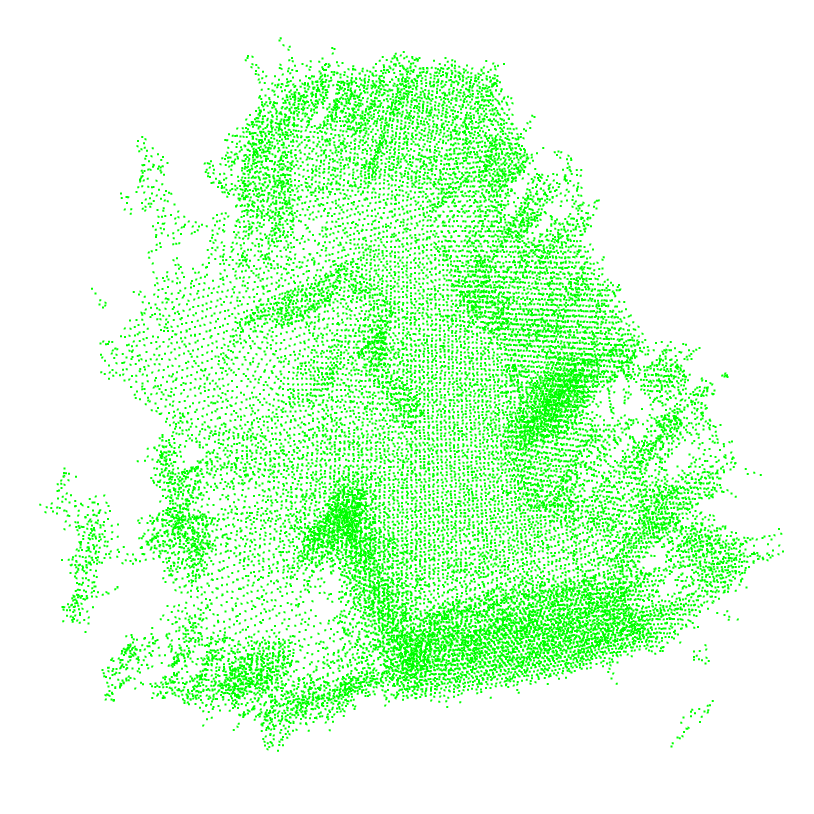
\includegraphics[width=\textwidth]{../img/v1-downsampled.png}
    \caption[Voxelised point cloud map]{Point cloud map voxelised to resolution 0.05 meter per voxel. Notice the regular spacing between points.}
    \label{fig:v1-downsampled}
\end{figure}

Algorithm for voxelisation is following. For each voxel (size of the voxel is determined by the resolution) we take all points contained in the voxel and approximate them with their centroid.

As discussed in section~\ref{chap:analysis}, in multi-robot system the down-sampling is typically performed by \gls{SLAM} algorithm running on each robot before publishing the map, thus saving bandwidth of the communication. However in typical situation we might want to reduce the resolution even further for the purpose of transformation estimation to reduce the computation time (for example each robot might publish a map with typical resolution $0.05$ meter per voxel, but for estimation we work with resolution just $0.1$ meter per voxel).

We show is the section~\ref{chap:evaluation} that our algorithm can reliable estimate the transformation when using $0.1$ meter per voxel resolution.

\subsection{Removing outliers}
\label{sec:outlier-removal}

Although the voxelisation can deal with some of the noise and inaccuracies, during experiments it has been beneficial to perform further outliers filtering to remove far laying points. Far-laying outliers may end-up being detected as keypoints, but they are usually not matched. Reducing the number of detected keypoints speeds up the later phases of estimation.

I have selected to use a simple radius-based outlier removal. This method searches for neighbours of each point within certain radius and removes points that have below threshold neighbours count.

Because descriptors of the outlier points are based on just a few points, which don't produce a robust matching candidates, and the radius outlier removal removes only the points with few neighbours, it does not reduce the robustness of the estimation.

For example on $2$ maps from \gls{AAU} dataset (see section~\ref{sec:aau-dataset}), outlier removal removes $326$ and $271$ points respectively ($7.29\%$, $6.16\%$), but number of detected keypoints decreases from $66, 63$ to $51, 56$ ($22.73\%$, $11.11\%$). Outlier removal didn't impact the estimation process negatively.

\subsection{Estimating surface normals}
\label{sec:normal-estimation}

The last preprocessing step is to estimate surface normals (figure~\ref{fig:v1-normals}). Surface normals are vectors perpendicular to the surface in the neighbourhood of the point. Surface normals are used in later steps to compute descriptors and by Harris keypoint detector.

\begin{figure}
    \centering
    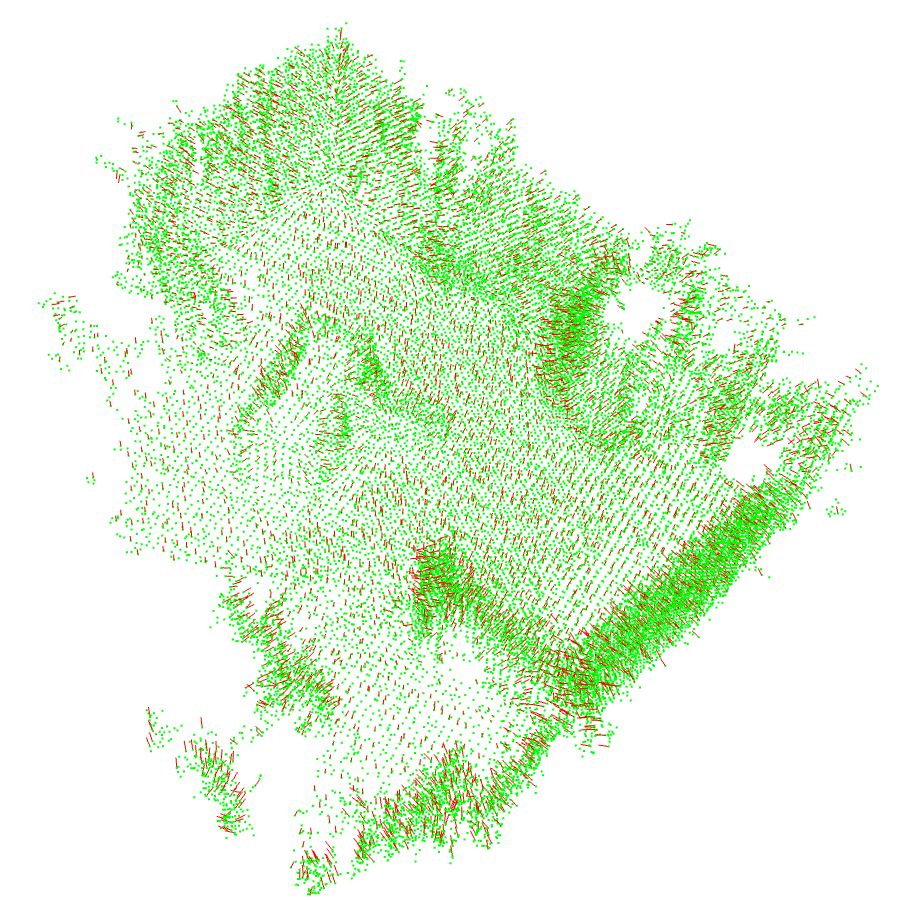
\includegraphics[width=\textwidth]{../img/v1-normals.png}
    \caption[Point cloud map with estimated surface normals]{Voxelised point cloud map with estimated surface normals (red). Only each fifth normal is visualised.}
    \label{fig:v1-normals}
\end{figure}

Algorithm for estimating surface normals is described by~\citet{RusuDoctoralDissertation}. The most important parameter for normals estimation is the size of the neighbourhood which is used for the estimation. This can be configured by the user.

\subsection{Detecting keypoints}
\label{sec:detect-keypoints}

Even after the down-sampling the maps contain usually too many points to work with all of them in later steps. We need to reduce the number of points further. Common technique used in the area of computer vision and robotics is to search for keypoints that identify suitable points for later matching (figure~\ref{fig:v1-keypoints}).

\begin{figure}
    \centering
    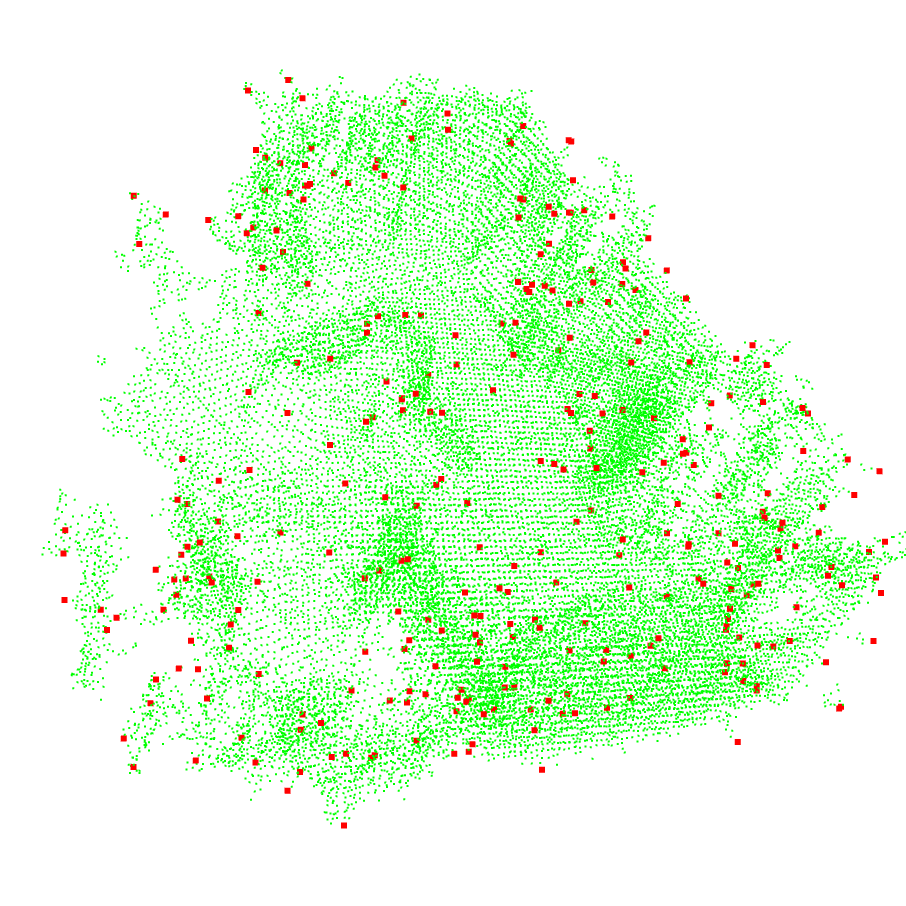
\includegraphics[width=\textwidth]{../img/v1-keypoints.png}
    \caption[Detected keypoints]{\gls{SIFT} keypoints (red) detected in the point cloud map (green).}
    \label{fig:v1-keypoints}
\end{figure}

There are two families of keypoints detectors that are being used with point clouds. Most of the approaches has been adapted from keypoints detectors that has been originally developed to work on images.

First class of detectors uses \gls{RGB} colour information stored for each point in the point cloud. This approach suppose that the point cloud has been obtained with detector that provide the colour information such as stereo rig camera setup, active \gls{RGB-D} cameras etc. For our approach we use \gls{SIFT} keypoint detector, which is an adapted algorithm from~\citet{lowe2004distinctive} that works on point clouds with \gls{RGB} information.

Second class of algorithms works with just geometrical information and is therefore able to work with point clouds that do not store any additional information for points. These algorithms can be used with point clouds composed of laser scans. Our algorithm implements Harris \gls{3D} keypoint detector for this purpose, which is an adapted algorithm from~\citet{harris1988combined}. Instead of using image gradients, which are not available in the point cloud without colour information, it uses surface normals, that capture geometrical properties of the point neighbourhood.

\subsection{Computing descriptors}
\label{sec:compute-descriptors}

Next step is to compute a local descriptor around each detected keypoint to be able to match keypoints between maps. Unlike the keypoint detection algorithms, algorithms for computing descriptors has been mostly designed from scratch to work on point clouds. Comprehensive review of the descriptors is given by~\citet{YasirThesis}.

Most of the descriptors does not use the colour information and use only local geometry around the point. Widely used \gls{PFH} descriptors, introduced by~\citet{rusu2008pfh}, use a multi-dimensional histogram with $125$ bins to provide an informative signature of a point neighbourhood. The histogram captures relationships between estimated surface normals (see section~\ref{sec:normal-estimation}). It uses relationships between all pairs of points in the neighbourhood and therefore has complexity $\bigO(k^2)$, where $k$ is number of points in the neighbourhood. There is a variant of \gls{PFH} descriptors \gls{PFHRGB} that stores also colour information in the extended histogram of $2 \times 125$ bins.

Main disadvantage of the \gls{PFH} descriptors is the high algorithmic complexity and therefore the slow processing speed~\citep{rusu2009fpfh}. Our implementation supports also \gls{FPFH}, introduced by~\citet{rusu2009fpfh}, \gls{SHOT} with colour, introduced by~\citet{tombari2011shot}, \gls{RSD}, introduced by~\citet{marton2010rsd}, and \gls{SC3D}, introduced by~\citet{frome2004sc3d}, novel descriptors which offer better processing speed compared to \gls{PFHRGB} and \gls{PFH}.

\subsection{Matching descriptors}
\label{sec:matching}

Next step in the pipeline is the descriptors matching, which yields an initial transformation estimate. It uses the features extracted from point clouds in the previous steps.

We match two sets of descriptors from two point clouds (figure~\ref{fig:v1-matching}). For each descriptors from the first set we want to find a descriptor in the second set, which describe the same place (in the second point cloud). This step is challenging, because the descriptors might be less descriptive than desired. Therefore the correct match might not be always the closest descriptor, but the $k$-nearest descriptor.

\begin{figure}
    \centering
    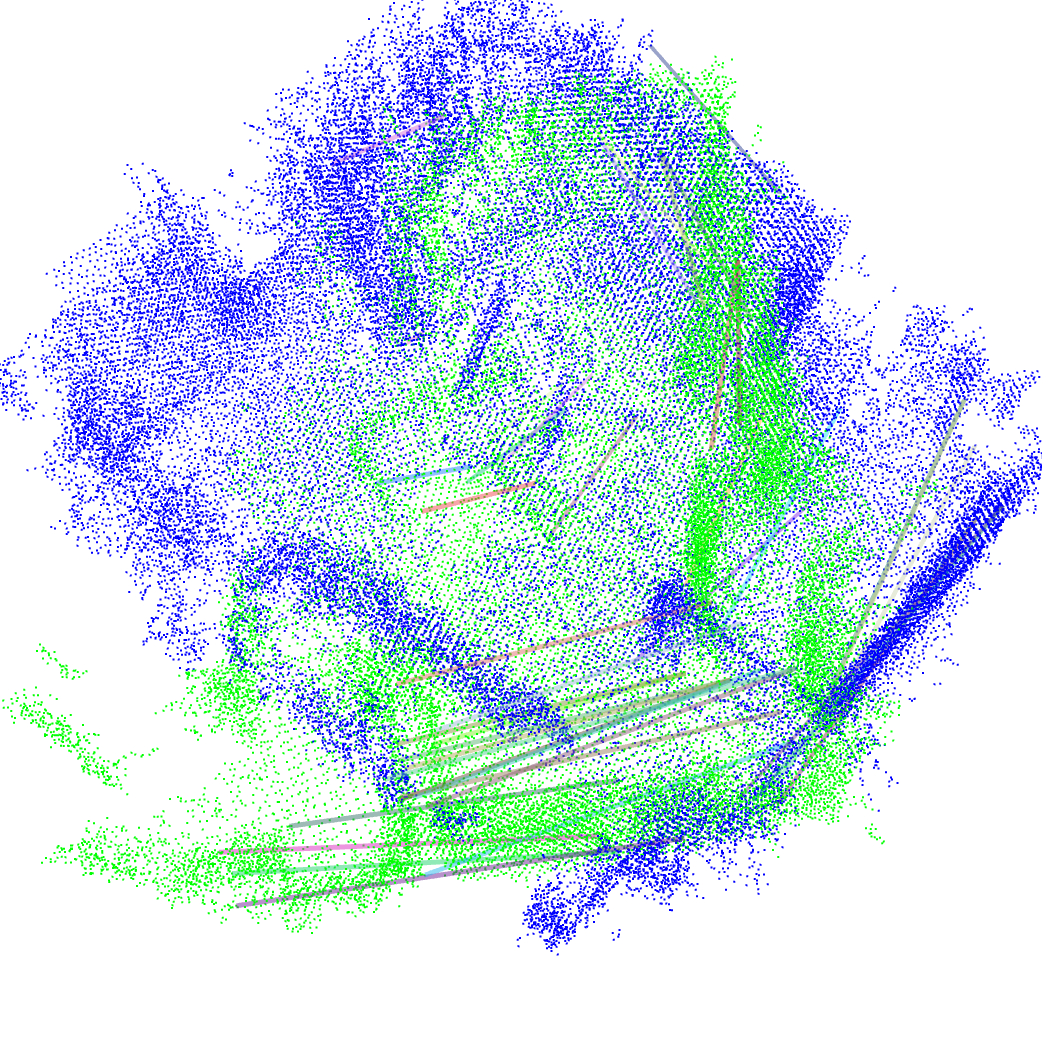
\includegraphics[width=\textwidth]{../img/v1-matching.png}
    \caption[Keypoint matches]{Matched keypoint descriptors between two point cloud maps (green, blue). Only inlier matches from \gls{RANSAC} are shown.}
    \label{fig:v1-matching}
\end{figure}

To overcome the issue, \gls{SAC-IA} algorithm has been proposed by~\citet{rusu2009fpfh} (algorithm~\ref{alg:sac-ia}).

\begin{algorithm}
    \caption[\gls{SAC-IA}]{\gls{SAC-IA} algorithm from~\citet{rusu2009fpfh}.}
    \label{alg:sac-ia}
    \begin{algorithmic}[1]
        \Require $D_1, D_2$ set of descriptors
        \Ensure rigid transformation estimate
        \Function{\gls{SAC-IA}}{$D_1, D_2$}
            \Loop~repeat $N$ times
                \State $K \gets$ draw $n$ descriptors from $D_1$
                \ForAll{$d_i \in K$}
                    \State $M \gets k$-nearest matches from $D_2$
                    \State $m_i \gets$ random sample from $M$
                \EndFor
                \State estimate rigid transformation for selected samples
                \State determine inliers
            \EndLoop
            \State \Return transformation with the most inliers.
        \EndFunction
    \end{algorithmic}
\end{algorithm}

The algorithm combines random matching of $k$-nearest descriptors and \gls{RANSAC} algorithm, introduced by~\citet{fischler1981ransac}.

% TODO describe why wanted the new algorithm

The algorithm was originally developed to work with \gls{FPFH} descriptors, that are fast to compute, but less descriptive that \gls{PFH}. With \gls{PFH} and \gls{PFHRGB} descriptors \gls{SAC-IA} sometimes yields sub-optimal transformation, even when there are good potential matches available in the descriptors sets, because it selects matching candidates randomly instead of preferring better matches. This lets us to development a new matching algorithm (algorithm~\ref{alg:cross-match}). This algorithm is deterministic to avoid problems caused by the randomness in \gls{SAC-IA}.

The algorithm is based on the idea of reciprocal match validation. When we are considering match $d_i \rightarrow d_j$, we try to match also $d_j \rightarrow d_i$. We consider all $k$-nearest neighbours for matching to deal with potential low descriptiveness and then select the best match with reciprocal match validation. We do not include \gls{RANSAC} in the scheme, output of the algorithm are just matched pairs of descriptors.

\begin{algorithm}
    \caption[Reciprocal $k$-nearest matching]{My matching approach using $k$-nearest matches validated with reciprocal matching}
    \label{alg:cross-match}
    \begin{algorithmic}[1]
        \Require $D_1, D_2$ set of descriptors
        \Ensure set of matches between $D_1, D_2$
        \Function{matchReciprocalK}{$D_1, D_2$}
            \State $M = \{\}$
            \ForAll{$d_i \in D_1$}
                \State $N \gets k$-nearest neighbours of $d_i$ in $D_2$
                \ForAll{$d_j \in N$}
                    \State $N' \gets k$-nearest neighbours of $d_j$ in $D_1$
                    \If{$d_i \in N'$}
                        \State $M \gets M \cup \{(d_i, d_j)\}$
                    \EndIf
                \EndFor
            \EndFor
            \State \Return $M$
        \EndFunction
    \end{algorithmic}
\end{algorithm}

Notice that our algorithm does not need any threshold for the maximum match distance and can therefore work with various kinds of descriptors without any need for a specific configuration. The only parameter is $k$ -- number of neighbours. As discussed in section~\ref{chap:evaluation} our approach shows better performance when there are enough good possible matches and is not influenced by randomness.

Both \gls{SAC-IA} and our reciprocal matching algorithm need to quickly find $k$-nearest neighbours. To achieve a good performance we use a approximative nearest neighbour search introduced by~\citet{muja2014flann}. This solution allows us to match large number of descriptors quickly, even though computational complexity rises significantly with $k$. During the experiments the matching step takes usually just a fraction of time needed to extract keypoints and descriptors.

\subsection{Estimating the final transformation}
\label{sec:final-estimation}

\gls{SAC-IA} embeds \gls{RANSAC} into its algorithm and therefore provides directly an initial transformation estimate. When we use our matching scheme as per algorithm~\ref{alg:cross-match}, we need to run \gls{RANSAC} step with rigid transformation model after the matching to get inlier matches. In the typical scenario most of the matches will be outliers, so without the \gls{RANSAC} step it would not be possible to estimate a consistent transformation.

\gls{RANSAC} transformation estimate is always based on the minimum number of points required to estimate the model (rigid transformation). To get better estimate for all inliers pairs we recompute the transformation estimate using least-squares on inlier pairs. We use \gls{SVD} to compute the new estimate, the technique is described by~\citet{golub1970svd}. Another widely used technique in Computer Vision is to use a non-linear least squares approach, such as Levenberg-Marquardt algorithm described by~\citet{more1978levmarq}, to optimize the transformation estimate re-projection error considering all inliers. Because we refine the transformation further with \gls{ICP}, there hasn't been any observed difference between using Levenberg-Marquardt or \gls{SVD}-based technique. The implementation uses \gls{SVD} to refine the transformation on inliers.

So far we have used only detected keypoints and descriptors computed around the keypoints to estimate the transformation. To refine the transformation using all the points in the point cloud we use \gls{ICP} algorithm introduced by~\citet{besl1992icp}. \gls{ICP} algorithm tries to minimize euclidean error distance between estimated corresponding points (figure~\ref{fig:v1-refined}). The estimated transformation from either \gls{SAC-IA} or the reciprocal matching scheme presented in section~\ref{sec:matching} is used as an initial guess for \gls{ICP}.

\begin{figure}
    \centering
    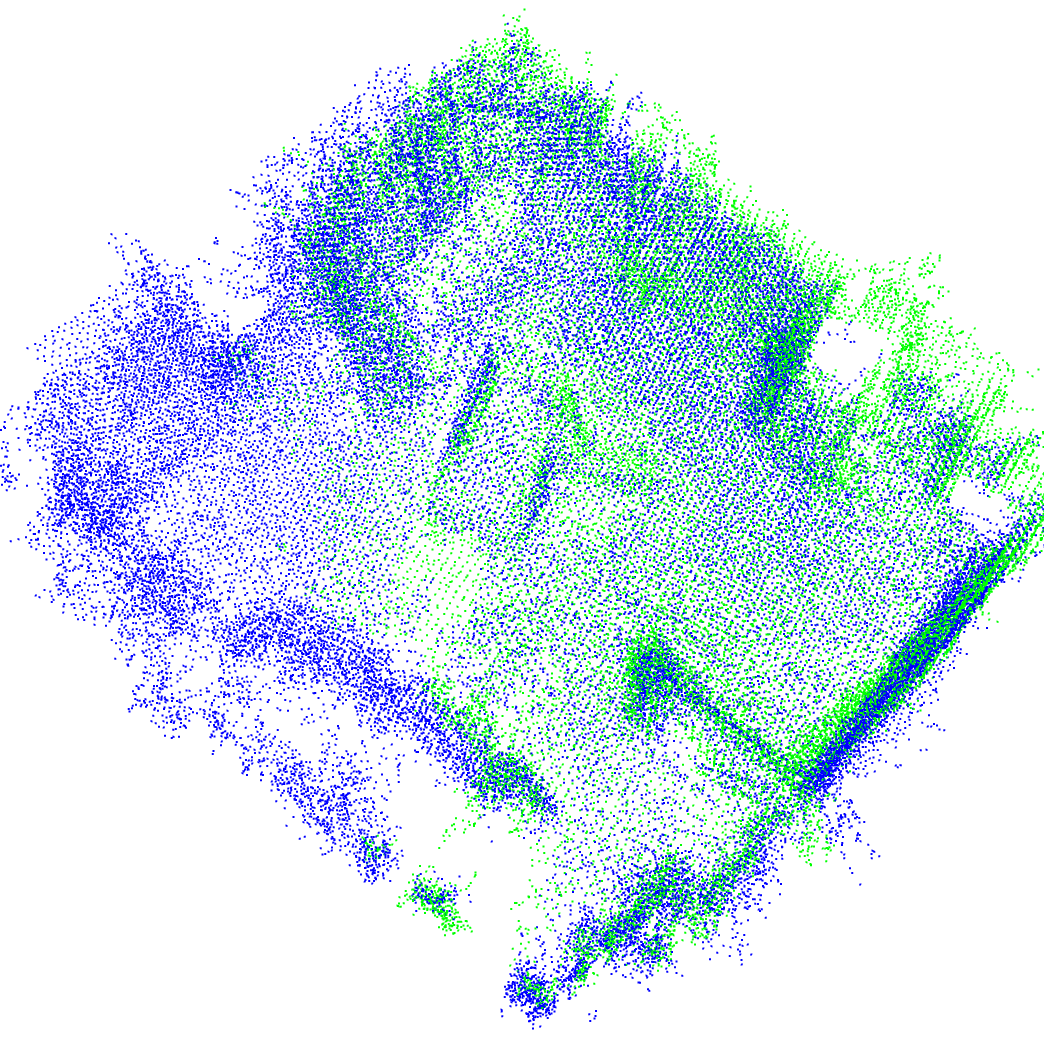
\includegraphics[width=\textwidth]{../img/v1-refined.png}
    \caption[Aligned point clouds]{Two point clouds maps (green, blue) aligned after refining initial transformation with \gls{ICP}. Initial transformation was computed from matches shown in figure~\ref{fig:v1-matching}.}
    \label{fig:v1-refined}
\end{figure}

The initial guess is usually close to the final transformation estimated by \gls{ICP}, especially when using the reciprocal matching algorithm~\ref{alg:cross-match} and \gls{RANSAC} for the estimation. Even though we use all the points with \gls{ICP}, because of the proximity of the guess to the final transformation only a couple of iterations is needed for \gls{ICP} to converge, so the refinement does not impact overall performance significantly.

Since the introduction of \gls{ICP} many \gls{ICP}-derived algorithms have been introduced to overcome issues associated with \gls{ICP}, especially to avoid local minima. A comprehensive review is given by~\citet{pomerleau2015reviewregistration}. Because our initial transformation is usually very close to the final transformation, the original \gls{ICP} algorithm performed well for our usecase during experiments.

\gls{ICP} refinement is the last step in estimating pairwise transformation. We use the output of the \gls{ICP} as the final estimated transformation between two maps.

\subsection{Evaluating the estimated transformation}
\label{sec:transform-evaluation}

To ensure robustness in real-world applications it is valuable to have a confidence measure for the estimated transformation. Commonly used measure for \gls{RANSAC}-based estimates is to use the number of inliers to access the algorithm performance. \citet{brown2007automatic} proposed a probabilistic model for image match verification based on the number of inliers. The authors used model with chosen $\alpha = 8.0$ and $\beta = 0.3$ given by equation~\eqref{eq:confidence-measure}, where $m$ is number of matches and $\psi$ is number of inliers in \gls{RANSAC}.

\begin{equation}
\label{eq:confidence-measure}
\frac{\psi}{8 + 0.3 \cdot m}
\end{equation}

Another possible confidence measure is to use distance error between the $2$ point clouds. This approach is common with point clouds and is implemented in \gls{PCL}. We typically use the Euclidean distance to have a natural metric estimate. This approach have two main issues. Because we do not know the correspondences between two maps we need to use the nearest neighbour for each point to compute the distance. Moreover to deal with occlusions (points outside intersection of the point clouds) we need to introduce cut-off threshold to deal with too large distances caused by points outside of the intersection.

In the implementation I use Euclidean distance to evaluate transformation estimate, because the implementation of \gls{SAC-IA} in \gls{PCL} does not provide information about inliers count.

% TODO write algorith for this?

\section{Estimating global transformations}
\label{sec:estimate-global}

Map-merging problem for two maps is discussed in section~\ref{sec:estimate-pair-wise}. To be able to merge more than two maps we consider a map-merging graph, definition~\ref{def:map-merging-graph}.

\begin{defn}[Map-merging graph]
    \label{def:map-merging-graph}
    A graph whose nodes correspond to robots' maps and whose edges represent pair-wise transformation estimates between the maps.
\end{defn}

To construct a map-merging graph for $n$ maps we need to estimate $\bigO(n^2)$ pair-wise transformations. Depending on the environment and maps relations map-merging graph might be dense of sparse, but typically will be missing some the edges, because some of the transformations could not be estimated, or could be estimated only with low confidence, see section~\ref{sec:transform-evaluation}.

Once we have constructed the map-merging graph, the global merged map can be computed by finding a spatial configuration of the nodes (maps) that is consistent with the transformations represented by the edges. In other words we want to find a transformation for each map from the global reference frame to the particular map consistent with the pairwise transformations.

\subsection{Map-merging as graph-based SLAM}

The idea of map-merging graph is similar to the idea of the pose graph used in graph-based \gls{SLAM}. Graph-based \gls{SLAM} uses a so-called graph-based formulation of the \gls{SLAM} problem. ``Solving a graph-based \gls{SLAM} problem involves to construct a graph whose nodes represent robot poses or landmarks and in which an edge between two nodes encodes a sensor measurement that constrains the connected poses.''~\citep{grisetti2010tutorial}.

In the graph-based \gls{SLAM} graph we have poses at different points in time, in the map-merging graph we have maps with origins in unknown positions. In the map-merging graph we associate our pairwise transformations estimates with edges and in the \gls{SLAM} graph we use usually direct sensor measurements. In both graphs we want to find the spatial configuration of the nodes of the graph that is the most consistent with constrains represented by the edges. If we are able to construct the map-merging graph (for which we need to do $\bigO(n^2)$ pair-wise transformation estimates), we can apply the graph-based \gls{SLAM} techniques on the map-merging graph to find the spatial configuration of the nodes that is consistent with our pair-wise estimates. Typically Gauss-Newton, described by~\citet{fletcher2013practical}, or Levenberg-Marquardt algorithm, described by~\citet{more1978levmarq}, are used to optimize the pose graph in graph-based \gls{SLAM}.

To support graph-based \gls{SLAM} approaches, there are libraries specifically focusing on graph optimization under constraints. Well-established examples include \texttt{G2O}, developed by~\citet{kummerle2011g2o}, and \texttt{TORO}, developed by~\citet{grisetti2007toro}. These libraries can be leveraged to solve the map-merging problem for $n$ maps.

\subsection{Solving map-merging problem without loop closures}

Graph optimizing techniques benefit from the presence of loop closures in the graph. During \gls{SLAM} mapping a loop closure occurs when the robot revisits a node in the graph. Loops in the map-merging graph require robot to be able to estimate pair-wise transformation with at least two neighbours. For example for the shortest loop in the graph, triangle with $3$ robots, we need each robot to be able to estimate both pair-wise transformations to remaining robots.

Loops in the map-merging graph will usually only occur in fairly large environments and when using many robots. Further on, unlike in graph-based \gls{SLAM}, loop closures may not be critical for good performance of the map-merging algorithm in the typical setup. In the \gls{SLAM} graph we expect measurements associated with the edges to be subject to the Gaussian noise and corrections based on loop closures are usually vital for good \gls{SLAM} performance. In the map-merging graph we have pair-wise estimates associated with edges based on the geometry of whole maps containing large number of points. The pairwise estimates tend to be quite precise, because they consider large portions of the environment. There are also available evaluation metrics for the pair-wise estimates (see section~\ref{sec:transform-evaluation}), which allow us to use only robust estimates in the graph.

Taking advantage of accurate pair-wise estimates in the map-merging graph we may avoid estimating all $\bigO(n^2)$ pair-wise estimates, especially since the pair-wise estimation is the most time-demanding step. To save time we can avoid pair-wise estimates introducing loops in the graph. We can stop pair-wise estimation when the nodes are within one connected component of the graph. We may want to employ a suitable heuristic for selecting the order of pair-wise estimates. Using this approach we might need just $\bigO(n)$ pair-wise estimates to estimate global transformations for the maps.

Below I present fast, non-iterative algorithm (algorithm~\ref{alg:global-transforms}) for extracting the global poses of maps from the map-merging graph suitable for use in such setup. The algorithm does not take any advantage of the loops in the graph (we expect the use with the approach mentioned above, which avoids loop closures). The algorithm, however, can work with graphs containing loops.

\begin{algorithm}
    \caption[Global poses extraction]{The algorithm to extract global poses of the maps from the map-merging graph (definition~\ref{def:map-merging-graph}).}
    \label{alg:global-transforms}
    \begin{algorithmic}[1]
        \Require weighted map-merging graph
        \Ensure Transformation for each map from global reference frame to the map reference frame
        \Function{extractGlobalPoses}{$G = (V, E)$ map-merging graph, $P_e \forall e \in E$ pair-wise transformations estimates}
            \State $C = (V_C, E_C) \gets$ largest connected component in $G$
            \State $T \gets$ maximum spanning tree of $C$ using confidences as weights
            \State $r \gets$ any node from $T$, selected as reference frame
            \State $E_s \gets$ edges of $T$ sorted by distance from $r$
            \State $A_r \gets I$
            \ForAll{$(i,j) \in E_s$}
                \State $A_j \gets A_i P_{(i,j)}$
            \EndFor
            \State $\forall i \not\in V_C: A_i \gets 0$
            \State \Return $A_0, A_1, \dots A_n$
        \EndFunction
    \end{algorithmic}
\end{algorithm}

Because only the maps in the same component of the map-merging graph can be related to the same reference frame, first step in the algorithm is to extract the largest connected component from the graph. In our setup we expect robots to ultimately form a one component and the transformations are computed only for this component. Remaining transformations are set to null transformation. If the robots are expected to operate for a longer period of time separately in multiple components, it might be beneficial for the coordination to compute transformations in all the components, each component having its own reference frame.

Next step in the algorithm is to extract the maximum spanning tree. The edges are weighted with estimated confidence for each pair-wise transformation, so that the most confident estimates are used. The possible loops are removed in this step and the non-tree edges are not used.

We can select any node from the spanning tree as the future global reference frame. All the transformations will be computed to this reference frame.

Last step is to compute the transformations to the selected reference frame. For computing the transformation of the node (map) we need transformations on the path from the reference frame (tree root) to the current node to be computed first (actually we need just the preceding transformation, but that implies computing all the transformations). To achieve this we can sort the edges by distance from the reference node, or just traverse the tree using \gls{BFS} or \gls{DFS} and compute the transformations during the traversal.


